\section{Methods}
\label{sec:method}

\subsection{Participants}
Thirty right-handed healthy subjects participated in this experiment (nine females, twenty-one males; age: 19$-$2.. years (mean =  years; S.E. =  years)). All the participants gave informed consent.\\
\\
Participants were primarily found amongst AI students at the Radboud University and other students from the Faculty of Social Sciences. Participants were excluded from the experiment when they exhibit certain symptoms or disorders, amongst epilepsy and dyslexia. The following exclusion criteria were used:
\begin{itemize}
	\item Cognitive deficits (or unfamiliarity with the English language) that made comprehension of the information letter and instructions difficult, or motor impairment that made comprehension of the task or pushing a button impossible.
	\item Epilepsy. Rapid serial visual presentation uses fast presented stimuli, so this criteria was added as a precaution.
	\item Dyslexia. We used artificial words in the experiment and the participant should have no trouble distinguishing between letters and registering the order of letters.
\end{itemize}

\subsection{Experimental paradigm}
%procedure
The experiment had a between subject design. To asses how well the subjects performed on artificial grammar learning using rapid serial visual presentation, we used three groups:
\begin{enumerate}
	\item The task was performed using three times 20 words for training and the stimuli were presented at a normal reading rate of 150 words per minute.
	\item The task was performed using three times 20 words for training and the stimuli were presented at a fast presentation rate of 450 words per minute.
	\item The task was performed using nine times 20 words for training and the stimuli were presented at a fast presentation rate of 450 words per minute.
\end{enumerate}

\noindent The participants were counter-balanced over groups. In each group were ten participants (group 1: six females, four males; age: ..$-$... years (mean = 22 years; S.E. = 2.4 years), group 2: one female, nine males; age ..$-$.. years (mean = 22.5 years; S.E. = 2.5 years), group 3: two females, eight males; age ..$-$... years (mean = 22.1 years; S.E. = 2.6 years)).\\
\\
%paradigm \& task
For each group the experiment followed the same structure (shown in Figure \ref{fig:timeline}) and started with a questionnaire. The participant was asked to fill out their age, gender, the number of languages they speak and their experience with speed reading on a scale from 1 (none) to 7 (usage on a regular basis). \\
\\
The participant had to perform three sessions in the experiment. The main task of the experiment is shown in Figure \ref{fig:tasktimeline}). The first session was a practice session to get acquainted with RSVP. The session began with the first three sentences of \textit{Beauty and the Beast} CITATION, at a rate of 150 words per minute. Hereafter, the participant was prompted that the rate would increase to 200 words per minute after a button press. Three to four sentences were presented for each rate, until 500 words per minute was reached.\\
The second session was the training session. This session differed between groups. The participants were unaware of differences between groups, and they did not know at which rate the words would be presented, the instructions were the same for all participants and only included that we would use one of the rates presented during practice. The training consisted of three or nine (depending on the condition) takes of 20 words, all from the grammar shown in Figure \ref{fig:grammar}. After every take there was time for a small break, so the participants would not get too weary to concentrate on the words.

\begin{figure}[h]
	\centering
	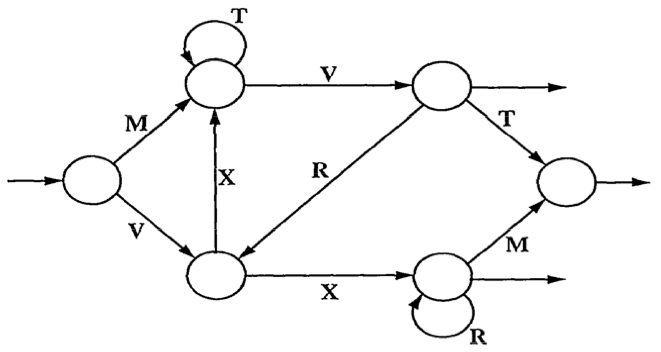
\includegraphics[width=0.45\textwidth]{media/grammar}
	\caption{Artificial grammar used for the experiment CITATION.}
	\label{fig:grammar}
\end{figure}

\noindent The third session was the test session. The participants were instructed that the words from the training session followed certain rules. Even though they did not learn these rules explicitly, they were asked to answer questions following their 'gut feeling'. The participant were then presented with 100 questions, all consisting of a word - either grammatical or nongrammatical - and the question whether they judged the word as grammatical or nongrammatical. There was a total of 50 words, equally many grammatical and nongrammatical words. Each word was represented twice in the questions to check for consistency. The response time and correct response rate were measured. After the task, the participant is asked to fill out a post-questionnaire containing one question: how he decided whether a word was ruleful or unruleful. This was used to decide which rules the participant used - if any.

\begin{figure}[h]
	\centering
	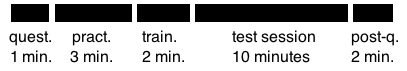
\includegraphics[width=0.45\textwidth]{media/timeline-experiment}
	\caption{This shows the estimated timeline, including small breaks, of the experiment.}
	\label{fig:timeline}
\end{figure}


\begin{figure}[h]
	\centering
	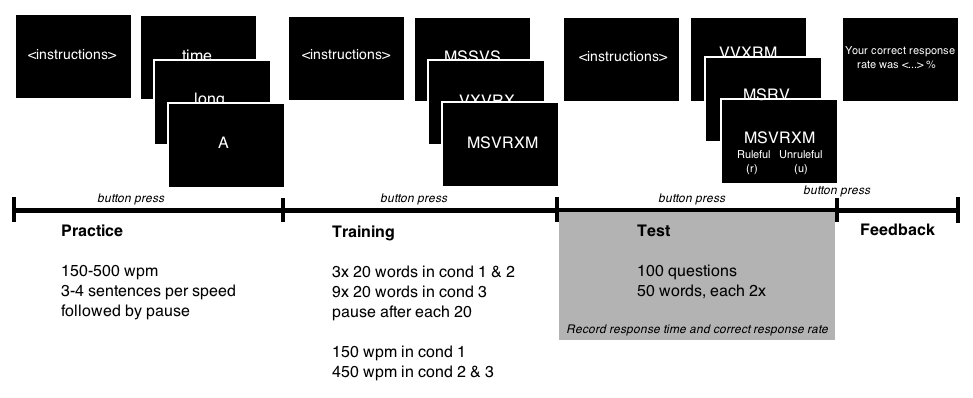
\includegraphics[width=\textwidth]{media/tasktimeline}
	\caption{This figure shows the timeline of the task. The task starts with the welcome screen with instructions about the practice session. The practice session starts at 150 words per minute and after each 3-4 sentences the participant is notified and the speed increases with steps of 50. After practice, instructions for the training session are given and the training starts after a countdown of 3 seconds. During the test session, no feedback is given, only after all questions are answered is the correct response rate given. This concludes the task.}
	\label{fig:tasktimeline}
\end{figure}

%feedback
\subsubsection{Feedback}
\label{sec:feedback}
In the experiment no feedback is given during the task. This is to ensure that the participants are not learning the rules during the test session and increasing performance for the remainder of the questions. Only after all questions are answered, the correct response rate is shown.

\subsection{Materials}
The experiment was done in a soundproof room with a desktop computer.
A program to execute the test as explained earlier was developed in Python using the PsychoPy package (\url{http://www.psychopy.org/}).
The stimuli that are based on the grammar as seen in Figure \ref{fig:grammar} and were used in the test can be found in Table \ref{tab:stimuli}.


\begin{table}[h]
\centering
\begin{tabular}{| p{3.5cm} | p{3.5cm} | p{3.5cm} |}
\hline
\textit{Training words} & \textit{Test words} & \textit{Test words}\\
\textit{(grammatical)} & \textit{(grammatical)} & \textit{(nongrammatical)} \\
\hline
& & \\
MSSSSV & MSSSV & MMVRX \\
MSSVS & MSSSVS & MSM \\
MSV & MSSV & MSRV \\
MSVRX & MSSVRX & MSRVRX \\ 
MSVRXM & MSV & MSSVSR \\
MVRX & MSVRXR & MSVRSR \\
MVRXRR & MSVRXV & MSVV \\
MVRXSV & MSVS & MXVRXM \\
MVRXV & MVRXM & MXVS \\
MVRXVS & MVRXR & MVRSR \\
VXM & MVRXRM & RRRXV \\
VXRR & MVRXVS & RVS \\
VXRRM & MVS & SSVS \\
VXRRRR & VXR & SVSSXV \\
VXSSVS & VXRM & SXRRM \\
VXSVRX & VXRRR & VRRRM \\
VXSVS & VXRRRM & VVXRM \\
VXVRX & VXSV & VXMRXV \\
VXVRXV & VXSSV & VXRRS \\
VXVS & VXSSSV & VXRS \\
          & VXV & VXRVM \\
         & VXVRX & VXX \\
          & VXVRXR & XRVXV \\
            & VXVRXV & XSSSSV \\
            & VXVS & XVRXRR \\
& & \\
\hline
\end{tabular}
\caption{Words used for the experiment.}
\label{tab:stimuli}
\end{table}


\subsection{Statistical analysis}

